%File: formatting-instruction.tex
\documentclass[letterpaper]{article}
\usepackage{aaai}
\usepackage{times}
\usepackage{helvet}
\usepackage{courier}
\usepackage{graphicx}
\usepackage{algorithmic}
\frenchspacing
\pdfinfo{
/Title (Zeno Problem Performance Analysis against Breadth First and A* Search Algorithms )
/Subject (AAAI Publications)
/Author (AAAI Press)}
\setcounter{secnumdepth}{0}  
 \begin{document}
% The file aaai.sty is the style file for AAAI Press 
% proceedings, working notes, and technical reports.
%
\title{Zeno Problem Performance Analysis against Breadth First and A* Search Algorithms}
\author{AbdulFatah Popoola \and
Majid Khonji\\
Computing and Information Science\\
Masdar Institute of Science and Technology\\
PO Box 54224, Abu Dhabi, UAE\\
Email: \{apopoola,mkhonji\} @masdar.ac.ae
}
\maketitle
\begin{abstract}
Search algorithms can be classified into two groups namely informed and uniformed search algorithms.
This paper seeks to evaluate the performance of an algorithm from each group based on varying
instances of a planning problem. We present empirical results showing the performance of breadth-first
and A* search algorithms in Zeno Travel, a STRIPS planning domain. We assumed that the
experiments are taking place in a deterministic, discrete, known and observable environment.
The motivation for choosing breadth-first and A* is because both algorithms are closely related in the way they carry out search.

\end{abstract}


\section{Introduction}
Planning - devising a plan of action to achieve goals - is a critical part of AI (Russell and Norvig 2010).
The process of looking for a goal in a plan is similar to searching for sequence of actions that solve a
problem. Planning problems can be formulated as consisting of a set of
states, an initial state, a goal test and a transition model. Search techniques can be then be employed on such models to solve planning problems.

Search algorithms basically take problem specifications – which are representations of the world – and
return a sequence of actions that lead to the desired goal. The solution generated depends on a couple of
parameters such as the representation model employed, the types of environments involved and the
variables present in the problem.

There are two major categories of search algorithms: uninformed and informed search. Uninformed
search algorithms, which do not distinguish between expanded states, exhaustively expand nodes
blindly until the goal is found. Informed search algorithms, however, employ heuristics in order to
detect goals more efficiently. We evaluated the performance of an algorithm from each category in this
paper; the algorithms evaluated were breadth-first search and A* search.

\subsection{Breadth First Search}
Breadth-first search, an uniformed search method, expands all nodes at a particular level in sequential
order before expanding the successors of the nodes at that level. It always expands the shallowest node
on the frontier (nodes that haven't been traversed but expanded). Breadth-first search is complete and
only optimal if the path-cost remains the same or doesn't decrease relative to the depth of a node. The
time and space complexity of breadth-first search are $O(b^d)$ and $O(b^d)$ respectively where $b$ is the
branching factor and $d$ is the depth at which the goal is found.

\subsection{A* Search}
A* attempts to find
the optimal solution path in a state-space graph. It evaluates the nearness of nodes to the goal state as a
function of $g(n)$, the total cost to get to that node from the initial state, and $h(n)$, the estimated heuristic cost
to get to the goal.
\begin{center}
$f(n) = g(n) + h(n)$
\end{center}
A* search always chooses the node with the smallest $f(n)$ value for expansion. The time and space
complexity of A* search are $O(b^d)$ and $O(b^d)$ respectively where $b$ is the branching factor and $d$ is the
depth at which the goal is found. A* is complete and optimal.

If the heuristic function $h(n)$ always evaluates to zero, then A* reduces to uniform-cost search, uniform-cost search is equivalent to breadth-first search for domains with uniform path cost. Hence A* can be said to be a form of breadth-first search.


\subsection{The Zeno-Travel Domain}
The STRIPS version of Zeno Travel, one of the domains used in the IPC-3, was used in this experiment. Zeno-Travel scenarios involve transporting people from one city to another. It involves cities, places, aircraft and varying fuel levels. The objective is to move people and the aircraft to various destinations.

Aircraft need fuel to fly between cities and can fly at two different speeds; however flying at high
speeds consumes more fuel. The actions available in this domain are 'board', 'debark', 'fly', 'zoom' and
'refuel'. The initial state includes a description of the location of the plane and all people and an ordering
of the various fuel levels, a specified number of objects, and the goal state specifies a destination for
the aircraft and all people.

The state-space of this problem is a function of the number of objects present in it and the branching-
factor is dependent on each state. Given $n$ cities, $a$ airplanes and $p$ people, the state-space complexity of the problem is 
\begin{center}
$O((n+a)^pn^a)$
\end{center}
This is because the maximum size of the state-space is $ (n+a)^p \times (6n)^a + 6 $. %TODO fix branching factor and state

In this paper, we carried out two different experiments on the Zeno-Travel domain. In the first experiment, we varied the number of cities while keeping the number of people and airplanes constant. In the second experiment, only the number of people in the problems changed. Different heuristics were employed in both experiments.

\section{Experiment Design}
The experiments involved comparing the performance of the breadth-first and A* algorithms on varying
problem specifications.The exponential complexity of both algorithms in the study, the large branching
factor of the search space and the huge state-space involved limited us to generating problems with
shallow trees – given the limited computational power at our disposal. This ensured that exhaustive
searches of the problem space always returned a plan on our low-end machines.
However in the second part of the experiment, we conducted minimal experiments on fully random problems with solutions at any level.

\subsection{Random Problem Generation}
The random problem generator was a simple program that handled the generation of random problem
files with varying properties. The input parameters include: the number of problem instances to create,
the search algorithm to use, the property to vary and the range of possible values of that property to
create.
Once all parameters were specified, the generator generated the files, ran the search algorithm on the
problems and wrote the results obtained to a file.

\subsection{Experiment 1: Varying number of cities}
\subsubsection{Heuristic function}
The heuristic used for the A* search was based on evaluating the number of literals in the goal state
that were satisfied in the initial state of a problem. This was used to calculate a weight to determine
how close a state was to the goal state. This heuristic is not always admissible but performs well, it
was chosen because the computational costs of admissible heuristics were quite high.
	%function heuristic returns h_score
%no of goal literals satisfied in initial state $
\begin{algorithmic}
	\STATE $count \gets num\_of\_goal\_literals\_satisfied\_in\_initial\_state$ 
	\IF {$count = zero$}
		\STATE $count \gets 0.00001$
	\ENDIF
	\STATE $h\_score \gets num\_of\_literals\_in\_problem\_initial\_state / count$

\end{algorithmic}
\subsubsection{Test 1:}
The problems generated in this test all had the same  goal state but contained varying number of
cities.
Since the goal was always at the same location in the graph irregardless of the problem, this experiment
investigates the performance of both algorithms under conditions of varying branching factors and
state-space size. A total of 500 problem files which contained a random number of cities were
generated. The number of cities ranged between 4 and 53 for each generated problem.

\subsubsection{Test 2:}
In the second test, we removed the simplifying assumption of unchanging goals. The problems
files used in this instance contained a varying number of cities and had changing goal states. This
enabled us to see the effects of varying branching factors, state-space size and goal states on the
performance of both algorithms. 500 problem files were also generated for this experiment and the
number of cities ranged between 4 and 53 for each problem file.

\subsection{Experiment 2: Varying number of people}
This experiment involved varying the number of people only. We generated around 100 random problems, changing the number of people
from 1 to 8. Roughly half of these problems were only solvable. We take the average of time and space for each group of problems with the same number of people.
A simple heuristic was used which returns the number of goal predicates that are not in a state. This is an admissible heuristic though.


\section{Results}
The average time and
space requirements of both search algorithms in both experiments were calculated and used to generate
plots.
\subsection{Varying number of cities}
\subsubsection{Test 1:}
Figure \ref{fig:avg_time_500_cities_constant_goal} and figure \ref{fig:avg_space_500_cities_constant_goal}

\begin{figure}[!htb]
	\centering
	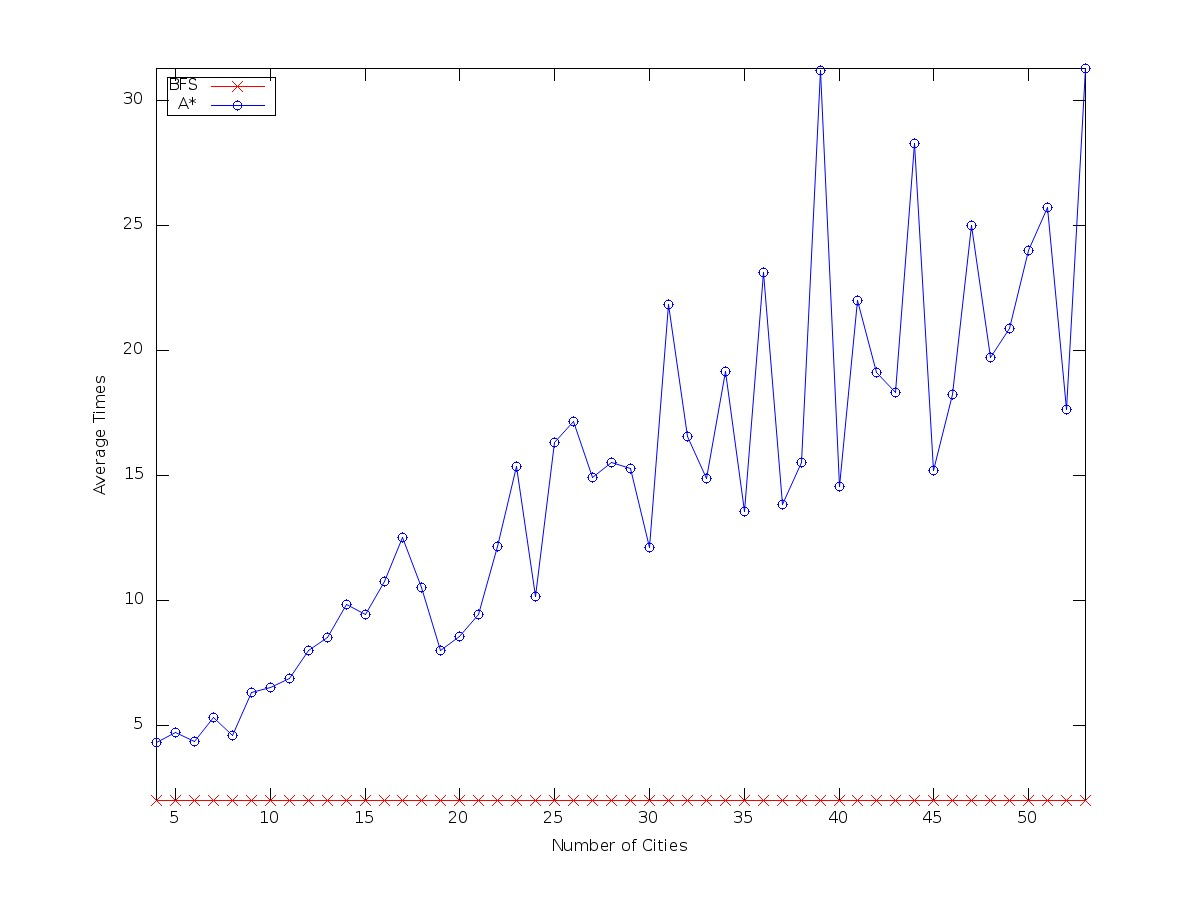
\includegraphics[scale=0.22]{./pics/avg_time_500_cities_constant_goal.jpg}
	\caption{Average time of 500 cities with a constant goal}
	\label{fig:avg_time_500_cities_constant_goal}
\end{figure}

\begin{figure}[!htb]
	\centering
	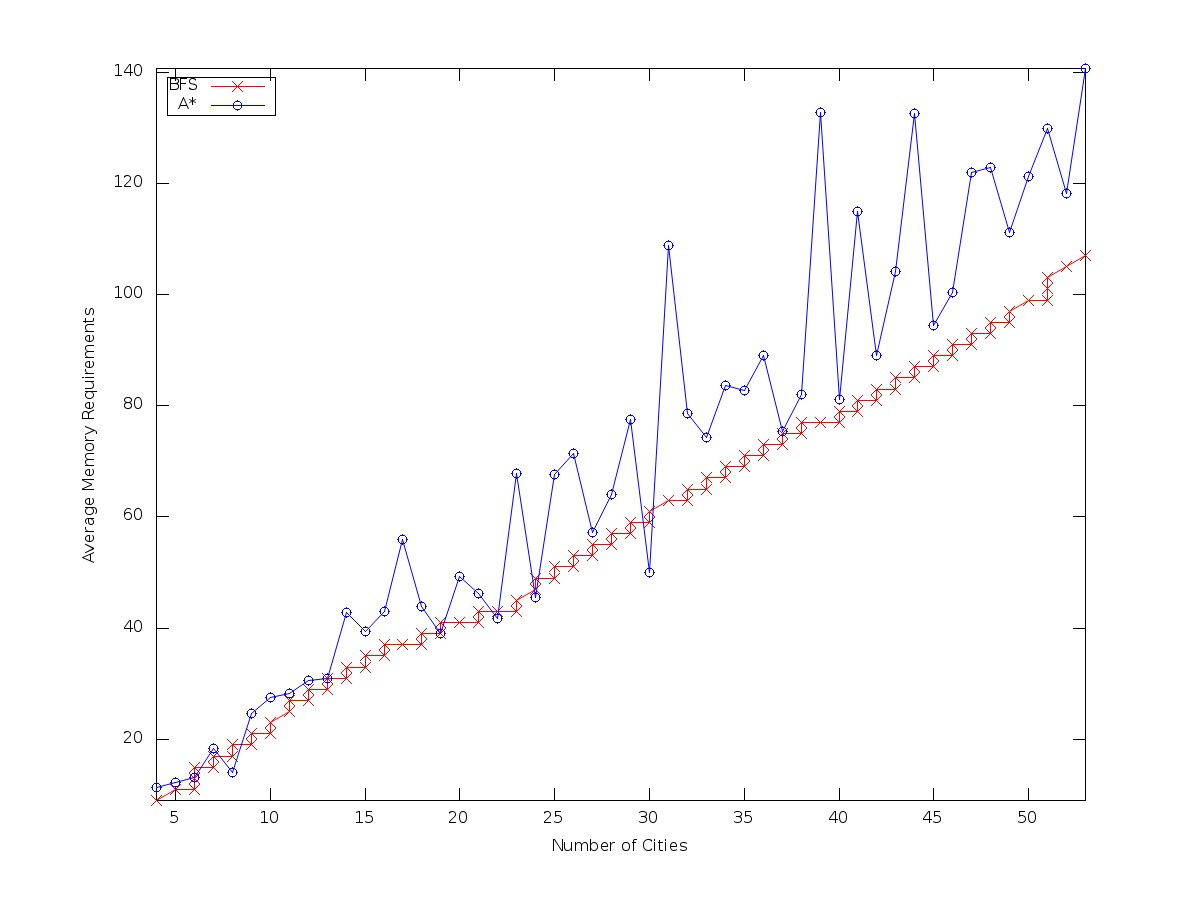
\includegraphics[scale=0.22]{./pics/avg_space_500_cities_constant_goal.jpg}
	\caption{Average space of 500 cities with a constant goal}
	\label{fig:avg_space_500_cities_constant_goal}
\end{figure}

\subsubsection{Test 2:}
Figure \ref{fig:avg_time_500_cities_random_goal} and figure \ref{fig:avg_space_500_cities_random_goal}


\begin{figure}[!htb]
	\centering
	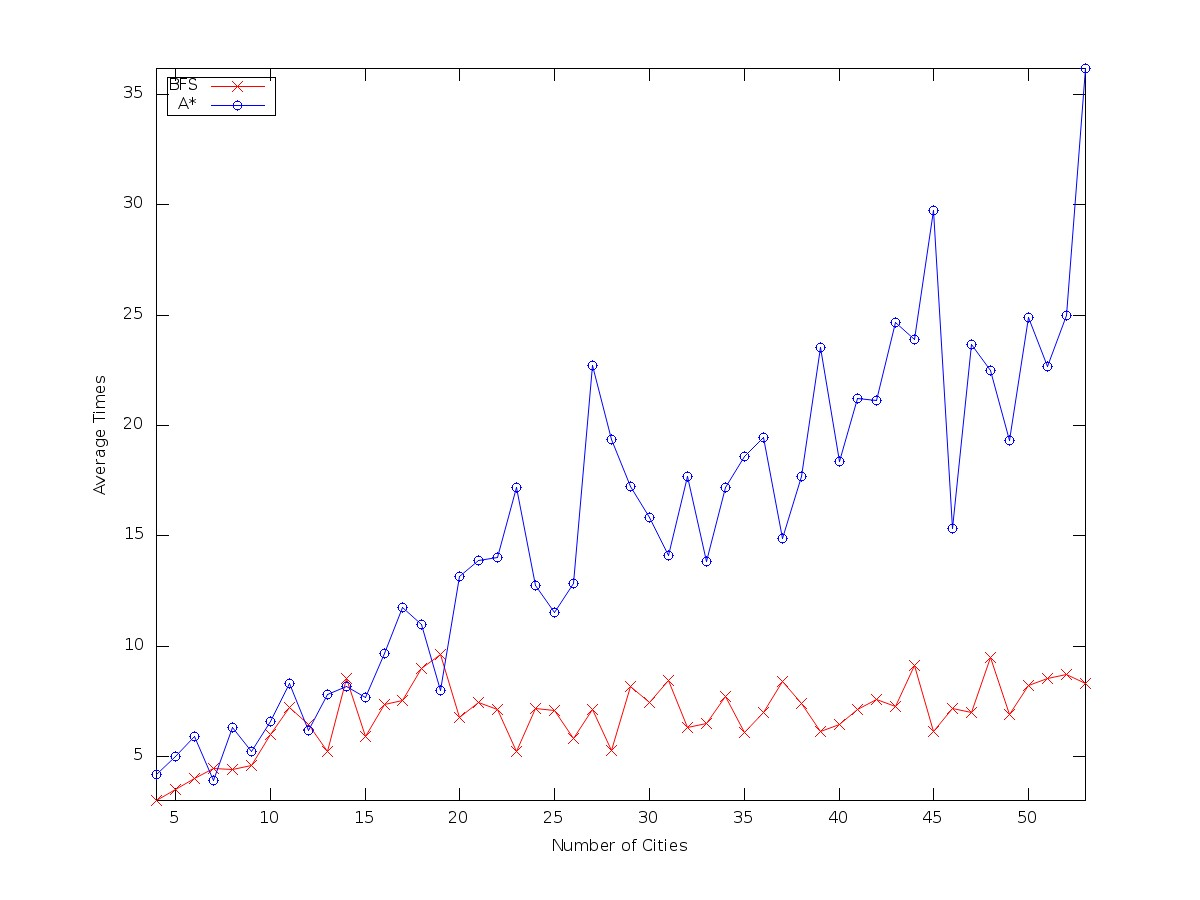
\includegraphics[scale=0.22]{./pics/average_time_500cities_random_goal.jpg}
	\caption{Average time of 500 cities with a constant goal}
	\label{fig:avg_time_500_cities_random_goal}
\end{figure}
\begin{figure}[!htb]
	\centering
	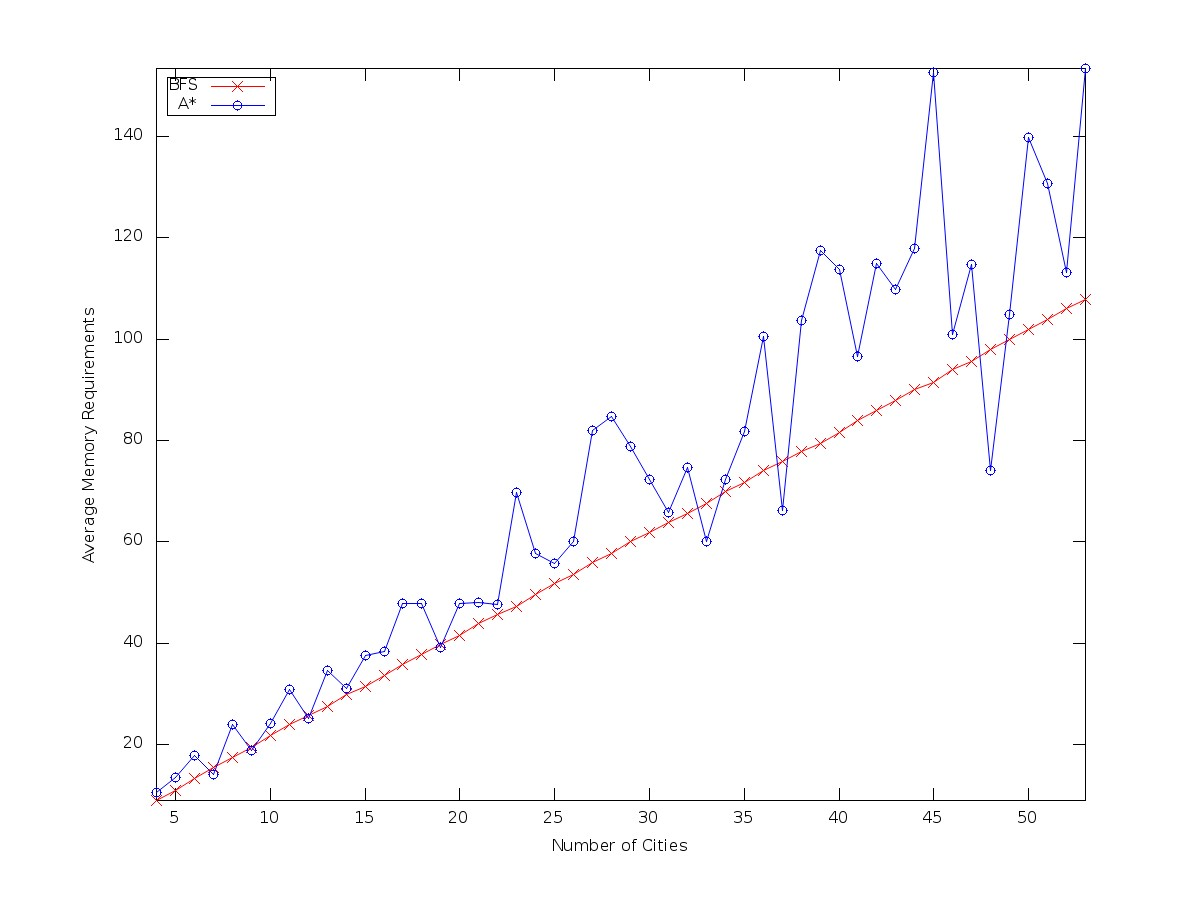
\includegraphics[scale=0.22]{./pics/avg_space_500_cities_random_goal.jpg}
	\caption{Average space of 500 cities with a random goal}
	\label{fig:avg_space_500_cities_random_goal}
\end{figure}
The graphs show that the breadth-first graph search consistently outperforms the A* search on shallow
domains.

\subsection{Experiment 2: Varying number of people}
Figure \ref{fig:time} show that A* is always faster than breadth first (i.e, visits less number of nodes). Figure \ref{fig:space}
show that A* also requires less space on average.
\begin{figure}[!htb]
	\centering
	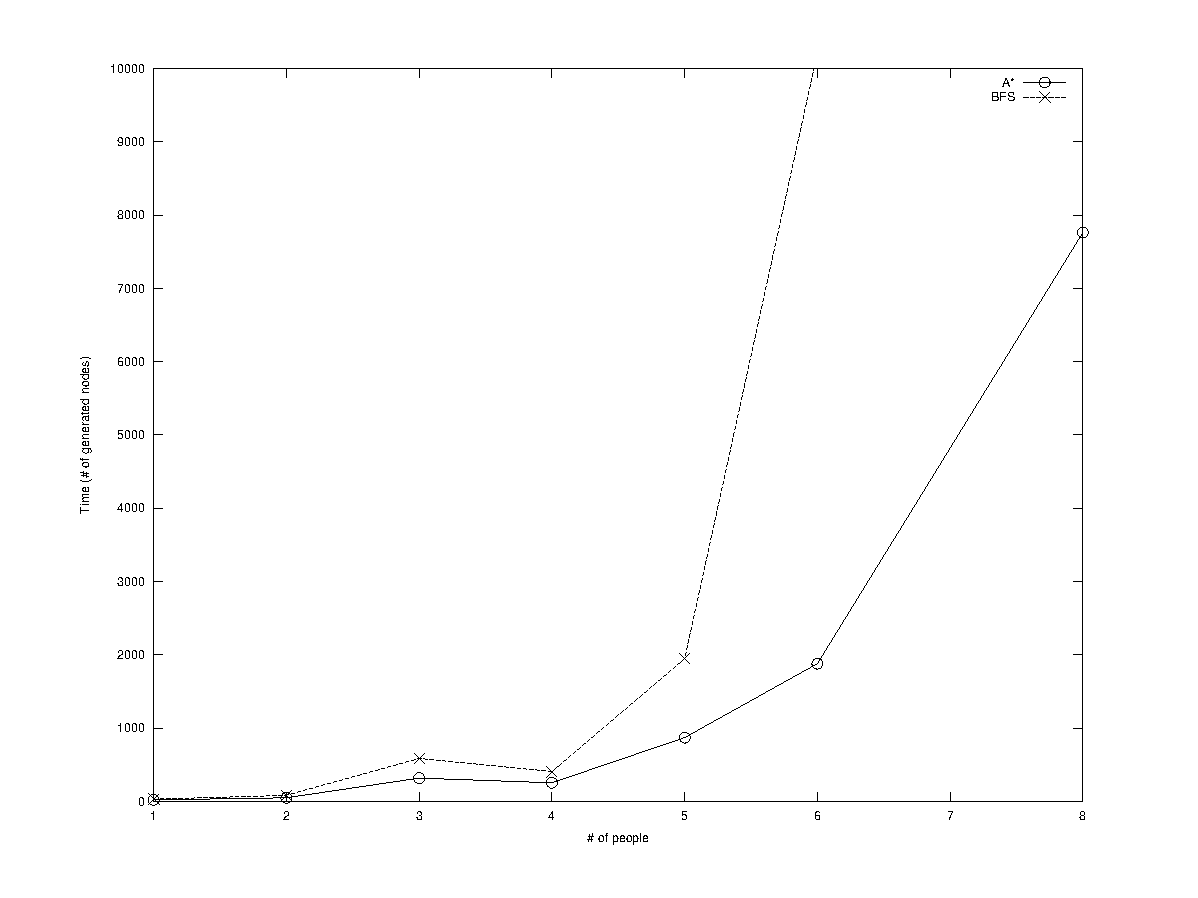
\includegraphics[scale=0.4]{./pics/time.pdf}
	\caption{Average Time of 100 problems (only solvable problems)}
	\label{fig:time}
\end{figure}
\begin{figure}[!htb]
	\centering
	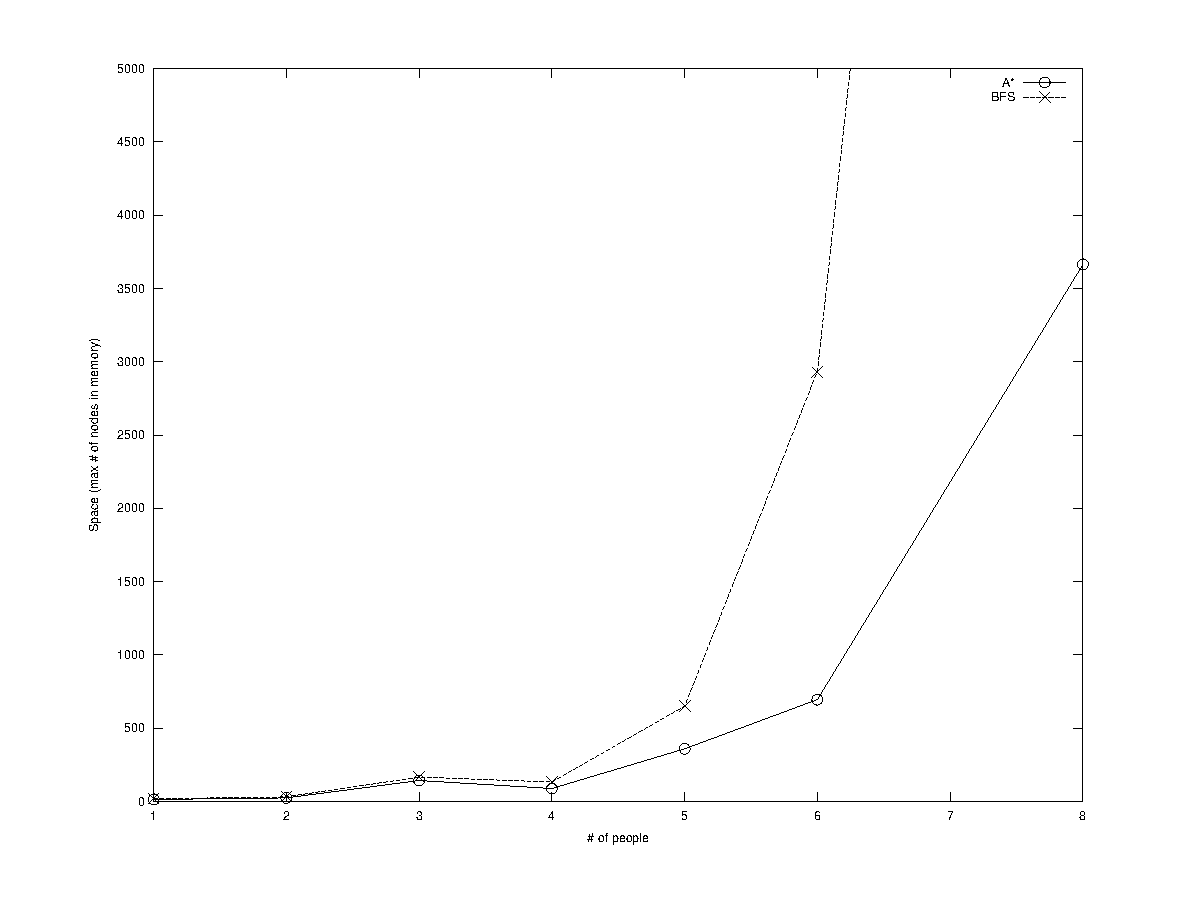
\includegraphics[scale=0.4]{./pics/space.pdf}
	\caption{Average Space of 100 problems (only solvable problems)}
	\label{fig:space}
\end{figure}

\section{Discussion and analysis}
\subsection{Experiment 1: Varying number of cities}
Multiple runs of the A* algorithm on the same set of result data showed varying time and memory
usage. This is due to the inadmissible heuristic which may have misled the A* search algorithm, consequently leading to changing memory and time requirements for the same problem specification. 
\subsubsection{Test 1:} 
Figure 1 shows the plots of the comparison average times. Given that the goal was always constant, the breadth-first took the same amount of time to locate the goal. However the heuristic function of A* led to it expanding arbitrarily more nodes in a bid to find the solution. This can be explained by A* propensity to search along the contour of the problem. However in both cases both of them found the optimal goals.
There is also a noticeable fluctuation in the range of values A* assumes after 25 cities.

Figure 2 shows the space requirements for both. A* search performance was quite good for small number of cities however as the number of cities increased, the performance of A* became more erratic and became worse. 
The breadth-first search consistently outperforms the A* search in both experiments in terms of
memory and time requirements. However the difference in performance between both algorithms is not
large and only becomes more pronounced as the number of cities approach 53.

\subsubsection{Test 2:}
The average time of breadth-first search increased steadily for increasing number of cities until it
leveled off at around 20 cities. After this, it maintained a relatively stable time for the remainder of the
study.
Similarly the A* started off quite well and performed even better than breadth-first search while the
number of cities were less than 20. However, a noticeable difference is observed once the number of cities got to 20 and after that, A* time requirements were never better than breadth-first search.
The space requirements for both algorithms grew steadily with increasing number of cities too.
Similarly there is a noticeable disruption in the average values of the A* search around the 20 – 25
cities range.

\subsection{Experiment 2: Varying number of people}
In this experiment, we used an admissible heuristic and got better results. The A* takes almost half of the time
taken by BFS, and similarly for the space as can be seen in Figures 5 and 6. Since the above experiment is quite computationally intensive, the number of samples
are quite small. But, the trend is quite obvious, A* is consistently better than BFS. The diagrams, shows some efficiency where
number of people is four. However, this is due to small sample size and the shallowness of the randomly-generated tree.

\subsection{Further analysis}
In a bid to explain the reason behind the disparity noticed in this performance of A* in the 20 – 25 city
threshold, we plotted all 500 values of space requirements on a single plot and got remarkable insights
(figure \ref{fig:500_varying_goal_compare_space}).

\begin{figure}[!htb]
	\centering
	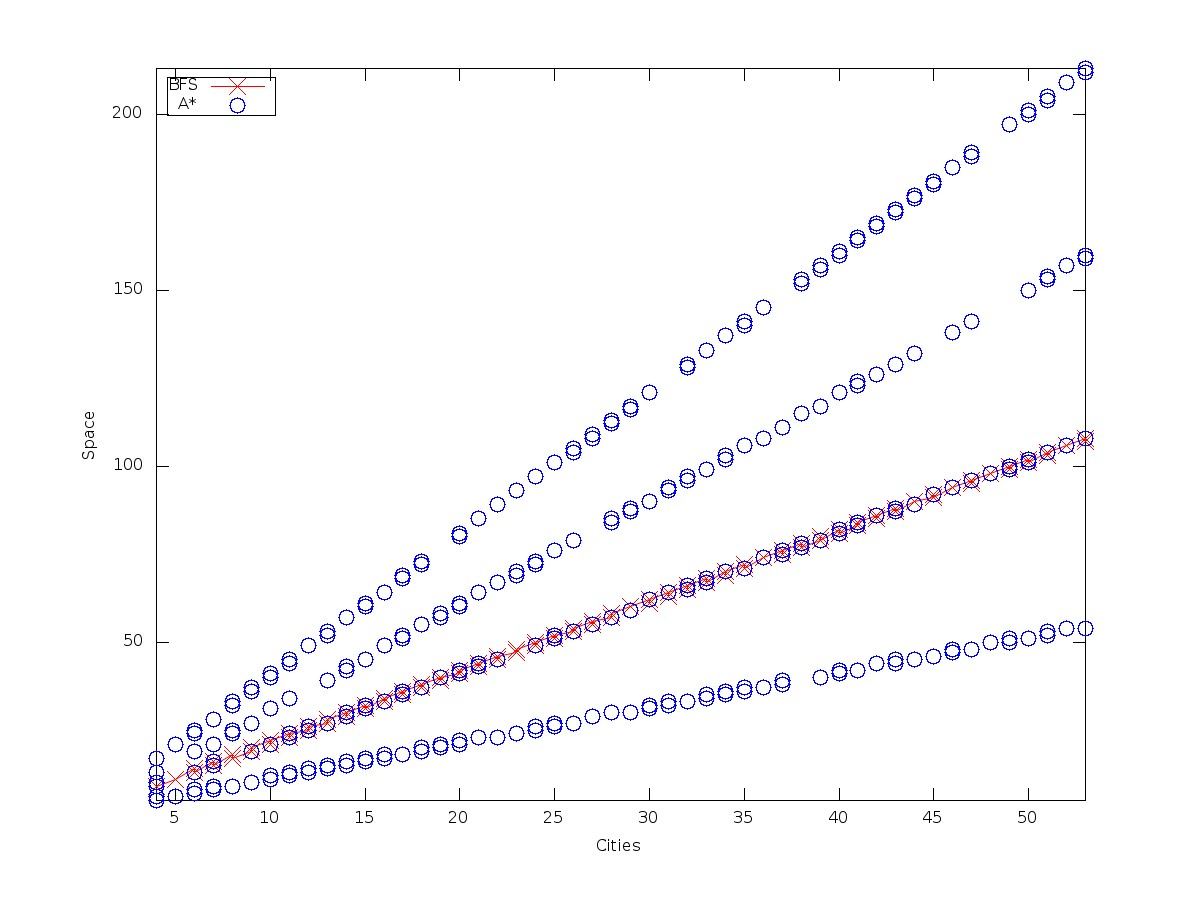
\includegraphics[scale=0.22]{./pics/500_varying_goal_compare_space.jpg}
	\caption{Varying goal space comparison}
	\label{fig:500_varying_goal_compare_space}
\end{figure}
The plot in figure 7 shows that the space requirements of A* search clearly separates into 4 lines; one of which is better
than BFS; one which matches it exactly and two others showing bad performance.
Given the random generation process and the varying number of cities and goal states, the number of
problem files generated (500) ensured that all possible numbers of cities between 3 and 53 are created.
Thus, there were instances of problems having the same number of cities but with varying goals. This
helps to explain the fact that the graph looks as it does. Down each city column, the only thing varying
was the goal states.

From this we can deduce that the A* search performed excellently given that the goal state of a city
was easily reached; this can be said to be due to the inadmissible heuristic employed in experiment 1. The heuristic function's inadmissibility became pronounced around the 20-25 city threshold and consequently affected the performance of A* search. However, the scope of this experiment didn't give us more
time to investigate deeper into this.


\section{Conclusion}
Throughout this work A* shows a better performance for both time and space whenever we use a good heuristic. On the other hand, it
could perform much worse if the heuristic was misguiding.
A potential future work would be testing different heuristics against time and space. In the case where we change the number of people, an
interesting heuristic would be: number of people who are not on-board and not in destination. It is always better to have many
passengers on-board than travelling people one by one.
Further studies can also be carried out on the issue of unsolvable random problems in the Zeno-Travel domain.

\section{Reference}
Russell S., and Norvig, P. 2010. \textit{Artificial intelligence: a modern approach.} Prentice Hall series in artificial intelligence. Prentice Hall.
\end{document}
